%-------------------
% CHAPTER 6: Design
%-------------------

\chapter{Design}

\label{chapter01}

With all the specification of the data the \thesis\ will work with, a good architecture for the system is needed. The whole software project is split in four different parts: Flights Availability Pipeline, User Searches Pipeline, Comparison Service and Web UI.
\\\\
In this chapter all four architectures for the four different parts will be defined and analyzed. All alternatives will also be defined and explain why it is not in the final architecture.
\\\\
Even so, first it is good to understand the general architecture of the whole \thesis.

%-----------------
%   SECTION 6.1
%-----------------

\section{Architecture}

The \thesis\ is split in very notable three layers: Data collection and processing, Comparison Server and Web UI. Two of this layer, server and user interface, suit exactly two of the four remarkable in the whole system, the Comparison Service and Web UI. Named the same to avoid confusion.
\\\\
An important characteristic of the \thesis\ is that the only way to feed the database is from the data collection and processing layer. This is different of most of projects and examples I have worked before in the University.
\\\\
The most common architecture used is a three layers (data layer, domain layer and presentation layer) where in the presentation layer the user could usually put data into the data layer. The \thesis\ work very different: The user interface (that is the presentation layer) does not put or modifies any data from the database. It only reads. The only way the database can be filled with valid data is from the \textit{data collection and processing layer}.

\begin{figure}[H]
\centering
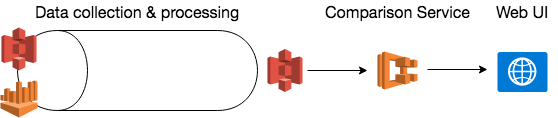
\includegraphics[scale=0.7]{diagrams/architecture01.png}
\caption{General view of the \thesis\ architecture}
\end{figure}

\subsection{Data collection and processing}

This layer is composed by two components, one for each data processing: Flights Availability Pipeline and User Searches Pipeline. The purpose of this layer is to collect all data necessary to do the comparison and filter and group according the final data model needed.
\\\\
Both components in the this layer uses very similar technologies. The data is read from different sources that already exist in \company\ and have a well defined design (\nameref{data_tribe} and \nameref{ingest_timetable_pipeline}) and services (\nameref{athena} and \nameref{s3}, S3). The whole data processing or data pipeline ran in Apache Spark, in an EMR cluster. In the end of the process both pipelines write into the same Storage service.

\begin{figure}[H]
\centering

\includegraphics[scale=0.7]{diagrams/architecture-data.png}
\caption{General view of the data collection and processing layer's architecture}
\end{figure}

\subsubsection{Amazon Athena} \label{athena}

\begin{figure}[H]

\includegraphics[scale=0.1]{resources/athena-logo.png}
\end{figure}

Amazon Athena\cite{athena}, is an Amazon Web Service that lets query data stored in \nameref{s3} (S3) using standard SQL\cite{sql}. It have no server running, so it have no infrastructure to manage.
\\\\
To access the data, Athena simply points to an S3 bucket with a defined schema and it lets you query its data with SQL queries. The cost of the service is based on the queries you run.
\\\\
\nameref{data_tribe} is responsible of creating schemas for Athena to read S3 buckets. They have a huge bucket called \texttt{grappler\_master\_archive} that contains all the user searches. Athena becomes the easiest way to access user searches data.

\subsubsection{Amazon Simple Storage Service} \label{s3}

\begin{figure}[H]

\includegraphics[scale=0.1]{resources/s3-logo.png}
\end{figure}

Amazon Simple Storage Service\cite{s3}, also known as \textit{S3}, stores data as objects within resources called buckets. It allows store unlimited objects in a bucket, also write, read and delete those objects. The maximum size of these objects is 5 terabytes. The access to buckets can be controlled.
\\\\
In \company, most of the results of \nameref{data_pipeline}s are stored as a single or multiple files in S3, then those are processed by \nameref{lambda} functions or other services. \squad\ stores timetables as a JSON\cite{json} file in its S3 bucket. Data tribe has also a bucket for user searches (and much more) data, but, as explained before, it provides access from \nameref{athena}.

\subsubsection{Apache Spark\textsuperscript{TM}} \label{apache_spark}

\begin{figure}[H]

\includegraphics[scale=0.1]{resources/apache-spark_logo.png}
\end{figure}

Apache Spark\textsuperscript{TM} is a unified analytics engine for large-scale data processing. It was created and it is currently maintained by the Apache Software Foundation\cite{apache_software_foundation}.
\\\\
Is one of the most popular fast and general-purpose cluster computing systems. It can run in a lot of different environments, Apache\textsuperscript{TM} Hadoop\textregistered\cite{hadoop}, Kubernetes\cite{k8s}, \nameref{emr} and much more. Spark provides four APIs: Java, Scala, Python, R and SQL. Over 80 high-level operators can help building parallel processes and can be called from most of its APIs. Both data pipelines are written using the Scala API.
\\\\
Apache Spark\textsuperscript{TM}'s architecture is based in \textit{Resilient Distributed Datasets}, RDD, a read-only multiset distributed in multiple machines. Those machines are based in the MapReduce paradigm, a programming model for big data dumps processing. Since the data is distributed, this process runs in parallel.

\subsubsection{Amazon Data Pipeline} \label{data_pipeline}

\begin{figure}[H]
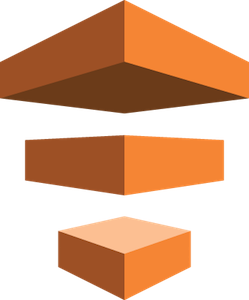
\includegraphics[scale=0.1]{resources/data_pipeline-logo.png}
\end{figure}

\subsubsection{Amazon Elastic MapReduce} \label{emr}

\begin{figure}[H]

\includegraphics[scale=0.1]{resources/emr-logo.png}
\end{figure}


%-----------------
%   SECTION 6.2
%-----------------

\section{Components}

%-----------------
%   SECTION 6.2
%-----------------


